\noindent
\section{On Complete graph}
\label{res_complete}
\noindent For {\bf complete graph} we assume the
number of nodes in the system to be $n$. 
%The time elapsed before the first sender (apart from the initiator) is created is represented by $t_1$ and the total diffusion time is denoted by $T^*$. We denote the expected values of these quantities by $% \mathbb{E}(t_1)$ and $\mathbb{E}(T^*)$ respectively. 
To determine how the number of
senders in the system changes with time, we plot the number of senders
against time for complete graph in Fig.~\ref{fig1}. 
%We further show in ~\ref{fig_k} how the diffusion progresses by plotting the number of nodes at each stage of infection at every time step for complete graph topology which roughly resembles epidemic process on a heterogenous population.  %Note
%that we assume the $d$-regular tree to be truncated with all the nodes except the leaf
%nodes have degree $d$.
We observe that the diffusion is initially slow which is then followed by a ramp-up after which the diffusion rate becomes almost exponentially fast.
To better analyze the process we divide the process into two phases i) the initial phase and ii) the residual phase. 


\noindent{\bf Initial phase:}  In the spreading process we define the initial phase to be the time between the
initiation and the point at which the first sender is created. We
define this as $t_1$; we will show later that $\hat E(t_1)$ (expected value of $t_1$) is
indeed an indicator for $\hat E(T^*)$ ($T^*$ - 
total diffusion time) in case of a complete graph.

Note that analytically deriving  $\hat E(t_1)$ assuming a  discrete 
(i.e., for a node the delay between two successive contacts is $1$ unit) diffusion model becomes severely complex and hence we adopt a continuous 
variant of the model. In fact, the calculation of the $\Pr \{ t_{1}=t\}$ can be treated as an expected time of filling the first urn with $k$
balls in the experiment where we have initially $d$ empty urns (degree of the node, for complete graph $d \sim n$) and at each
single time step we add a single ball to one urn chosen randomly. 
 For any $k$%
-parts message, by~\cite{kaplan1977generalization} we describe our problem
as a unit-time Poisson process. Note that for a poisson process the inter-arrival time follows exponential distribution ($\lambda$) and expected number of arrivals in time $t$ is $\lambda t$.  
 Let 
$X_{j}(t)$ be a random value describing the number of balls in $j^\textrm{th}$ urn up
to time $t$. More precisely $X_{j}(t)=\sum_{i=1}^{N}1$ where $N$ is a random variable 
with Poisson distribution $\mathcal{P}(\frac{t}{d})$. Essentially $N$ represents number of draws
of the $j^\textrm{th}$ urn up to time $t$ if $d$ urns exist in the system.
Hence $\{X_{j}(t)\}$s are i.i.ds and $X_{j}(t)\sim\mathcal{P}(\frac{t}{d}%
) $.  
{We formulate the analytical result for complete graph topology through the following theorems 1-5. The various notations are further 
summarized in table \ref{tab:1}}



\begin{theorem}
%\vspace{-.2cm}
For a message with $k$ tokens, the expected value of $t_1$, 
$\hat E(t_{1})=\int_{0}^{\infty}(1-P(t_{1}\leq
t))dt = \int_{0}^{\infty}Q(k,\frac{t}
{d})^{d}dt$
where $Q(k,u)$ is a regularized incomplete gamma function and $d$ is the degree. 
% Furthermore for fixed $i\geq 2$ the random variable $t_{i}d^{-\frac{k-1}{k}}$ converges to a limiting random variable $\tau _{i}$ and the following recursion holds for the expectations: $\frac{\mathbb{E}\left( \tau _{i}\right) }{\mathbb{E}\left( \tau _{i-1}\right) }%=1-\frac{2k-1}{ik} .$
\label{theorem-0}
\end{theorem}

\begin{proof}
 \begin{equation}
\begin{aligned} 
\hat E(t_{1})=&\int_{0}^{\infty}(1-P(t_{1}\leq
t)dt=\int_{0}^{\infty}(1-(1-P(t_{1}
>t))dt\\=&\int_{0}^{\infty}P(X_{j}(t)<k)^{d}dt=\int_{0}^{\infty}Q(k,\frac{t}
{d})^{d}dt\label{eqint} 
\end{aligned}
\end{equation}

where $Q(k,u)$ is a regularized incomplete gamma function i.e. 
\begin{equation}
Q(k,u)=\frac{\Gamma(k,u)}{\Gamma(k)}=e^{-u}\sum_{l=0}^{k-1}\frac{u^{l}}{l!}
\end{equation}
is valid for any natural $k$ and non-negative $u$.

\end{proof}

%\vspace{-.2cm}
Note that $t_{1}$ for a Poisson process, is a continuous random variable. 

\noindent{\bf Residual phase:} We next proceed to establish the relation between $\hat E(t_1)$ and $\hat E(T^{*})$. Apart from assuming the continuous model, 
we compute scaled $t_1$ and $T^{*}$ (by $d^{\frac{k-1}{k}}$, 
(this specific scaling function was initially calculated for $k=2$ and then generalized for higher values)) instead of their explicit values to further aid our analysis. 
To summarize, we start by computing  
expected values of scaled $t_1$ and $T^{*}$ considering a continuous (Poisson) model with $d\rightarrow \infty$ and show that the results hold for finite $d$. Finally we show that the results for the continuous model extend to the discrete model.
We begin by showing that $t_1$ (time to create the first sender apart from the initiator) is an indicator for the diffusion delay $T^*$ through the following two theorems. 
%The detailed proof of both the theorems are available in the supplementary.


\begin{table}
\centering
\caption{Summary of the notations used.}
\label{tab:1}
\scalebox{0.65}{
\begin{tabular}{|l|l|}
\hline
{\bf Symbol}             & {\bf Definition}                                                                     \\ \hline\hline
$t_1$              & Time between initiation and creation of first sender                           \\ \hline
$T^{\ast}$         & Total diffusion time                                                           \\ \hline
$\hat E(t_1)$      & Expected $t_1$ (obtained analytically)                                         \\ \hline
$\hat E(T^{\ast})$ & Expected $T^{\ast}$(obtained analytically)                                     \\ \hline
$Av(t_1)$          & Expected $t_1$ (obtained empirically)                                          \\ \hline
$Av(T^{\ast})$     & Expected $T^{\ast}$ (obtained empirically)                                     \\ \hline
$s_1$              & Limiting random variable of $t_{1}d^{- \frac{k-1}{k}}$as $d\rightarrow \infty$ \\ \hline
$\tau_i$           & Scaled time span between creation of $(i-1)^{th}$ sender and $i^{th}$ sender   \\ \hline
$s^{\ast}$         & Limiting random variable for $T^{\ast}d^{-\frac{k-1}{k}}$                      \\ \hline
\end{tabular}}
\end{table}

\begin{theorem}
%\vspace{-.2cm}
For a message with $k$ tokens the random variable $t_{1}d^{-\frac{k-1}{k}}$
converges as $d\rightarrow \infty $ to a limiting random variable $s_{1}$
with density $\frac{x^{k-1}}{(k-1)!}e^{-\frac{x^{k}}{k!}}$ 
and expectation $%
\hat E \left( s_{1}\right) =(k!)^{\frac{1}{k}}\Gamma\left(1+\frac{1}{k%
}\right).$ 
% Furthermore for fixed $i\geq 2$ the random variable $t_{i}d^{-\frac{k-1}{k}}$ converges to a limiting random variable $\tau _{i}$ and the following recursion holds for the expectations: $\frac{\mathbb{E}\left( \tau _{i}\right) }{\mathbb{E}\left( \tau _{i-1}\right) }%=1-\frac{2k-1}{ik} .$
\label{theorem-1}
\end{theorem}
%\vspace{-.2cm}

\begin{proof}
 The proof is based on Poisson clock approximation approach
introduced {previously.} 
% which means that variables are
% independent and for a price of acceptable level of error of the order $%
% o_d(1) $. 
We start from the calculation of the CDF for the random variable $%
t_1 d^{-\frac{k-1}{k}}$:


\begin{equation}
\begin{aligned} &F_{t_1 d^{-\frac{k-1}{k}}}(x)=P(t_1 d^{-\frac{k-1}{k}}\leq
x)\\
%=1-P(t_1>xd^{\frac{k-1}{k}})\\
%&=1-P(X_j(xd^{\frac{k-1}{k}})<k)^d
&=1-Q(k,\frac{xd^{\frac{k-1}{k}}}{d})^d%
\\
&=1-\left(\sum_{i=0}^{k-1}e^{-xd^{-\frac{1}{k}}}(xd^{-%
\frac{1}{k}})^i/i!\right)^d\\ \label{eq-prof-1}
%&=1-\left(1-e^{-xd^{-\frac{1}{k}}}(xd^{-%
%\frac{1}{k}})^k/k!(1+o(1))\right)^d 
 \end{aligned}
\end{equation}

where in the last line we used the common simple approximation of Poisson
cumulative distribution in long tail.

Since we are interested in limits as $d\rightarrow \infty$, for $%
exp(-xd^{-\frac{1}{k}})\rightarrow 1$ and we can compute limits of $F_{t_1
d^{-\frac{k-1}{k}}}$ 
as follows: 
\begin{equation}
\begin{aligned} F_{s_1}(x)&=\lim_{d\rightarrow\infty}F_{t_1
d^{-\frac{k-1}{k}}}(x)\\&=\lim_{d\rightarrow\infty}1-\left(\sum_{i=0}^{k-1}e^{-xd^{-\frac{1}{k}}}(xd^{-%
\frac{1}{k}})^i/i!\right)^d \\&=
1-e^{(-x^k/k!)} \label{eq-prof-cdf1} \end{aligned}
\end{equation}

Now, the density function of $\tau_1$ can be calculated as - 

\begin{equation}
f_{s_1}(x)=\frac{dF_{s_1}}{dx}(x)=\frac{x^{k-1}}{(k-1)!}exp%
\left(-\frac{x^{k}}{k!}\right)
\end{equation}
Further the expectation of $s_{1}$ is - 
 \begin{equation}
\begin{aligned}
\hat E(s_1)&=\int_{0}^{\infty}xf_{s_1}(x)dx=\int_{0}^{\infty}%
\left(uk!\right)^{\frac{1}{k}}e^{-u}du\\&=\left(k!\right)^{\frac{1}{k}}%
\int_{0}^{\infty}u^{\frac{1}{k}}e^{-u}du=\left(k!\right)^{\frac{1}{k}}\Gamma%
\left(1+\frac{1}{k}\right) \label{e-tau-1} 
\end{aligned}
\end{equation}
\end{proof}



We next compute the expectation of the (scaled) time $%
T^{\ast }$ till all nodes become senders.  
We consider $T_{i}=t_{i}d^{-\frac{k-1}{k}}$. We further assume $\tau _{i}$ as the
scaled time span between the creation of $(i-1)^\textrm{th}$ new sender and that of $i^\textrm{th}$ new
sender. Correspondingly $\tau _{i}^{\ast }$ represents the scaled time for
the original process where every node with at least $k$ tokens acts as a
sender node.  
We have $\hat E\left( \tau _{i}^{\ast }\right) =%
\frac{1}{i}\hat E\left( \tau _{i}\right) =\frac{1}{i}\left( \hat E%
\left( T_{i}\right) -\hat E\left( T_{i-1}\right) \right)$.  
Note that $\tau _{1}$ is equal to $T_{1}$ as $T_{0}$ is 0 and hence $\hat E(s_1)$ equals $\hat E(\tau _1)$.
%\vspace{-.2cm}
\begin{theorem}
%\vspace{-.2cm}
\label{theorem-2} $T^{\ast }d^{-\frac{k-1}{k}}$ converges to a limiting
random variable $s^{\ast }$ with 
%\vspace{-.2cm}
\begin{equation*}
\vspace{-.3cm}
\hat E \left( s^{\ast }\right) =\sum\limits_{i=1}^{\infty }\hat E%
\left( \tau _{i}^{\ast}\right) = \hat E(\tau_1)\frac{k}{k-1}
\end{equation*}
\end{theorem}

\begin{proof}
$G_{i}^{\left( d\right) }\left( z\right)
=1-F_{i}^{\left( d\right) }\left( z\right) =\Pr \left\{ t_{i}>zd^{\frac{k-1}{%
k}}\right\} =\Pr \left\{ T_{i}>z\right\} $(complementary cdf of $T_i$). Since $\frac{zd^{\frac{k-1}{k}}}{%
d}=zd^{-\frac{1}{k}}$ we have 
\begin{equation}
\begin{aligned} G_{i}^{\left( d\right) }\left( z\right)
=&\sum_{j=0}^{i-1}\binom{d}{j}\left( \sum_{l=0}^{k-1}\frac{1}{l!}\left(
zd^{-\frac{1}{k}}\right) ^{l}e^{-zd^{-\frac{1}{k}}} \right)
^{d-j}\\&\left( 1-\sum_{l=0}^{k-1}\frac{1}{l!}\left(
zd^{-\frac{1}{k}}\right) ^{l}e^{-zd^{-\frac{1}{k}}} \right)
^{j} \\
%=&\sum_{j=0}^{i-1}\binom{d}{j}\left( 1-\left( 1+o_{d}\left( 1\right)
%\right) \frac{z^{k}d^{-1}}{k!}e^{-zd^{\frac{-1}{k}}}\right) ^{d-j}\\&\left(
%\left( 1+o_{d}\left( 1\right) \right)
%\frac{z^{k}d^{-1}}{k!}e^{-zd^{\frac{-1}{k}}}\right) ^{j} \\
%=&\sum_{j=0}^{i-1}\frac{d^{j}}{j!}\left( \frac{z^{k}}{k!}\right)
%^{j}\frac{1}{d^{j}}e^{-\frac{z^{k}}{k!}}\left( 1+o_{d}\left( 1\right)
%\right) \\
=&\sum_{j=0}^{i-1}\frac{1}{j!}\left( \frac{z^{k}}{k!}\right)
^{j}e^{-\frac{z^{k}}{k!}}\left( 1+o_{d}\left( 1\right) \right) 
\end{aligned}
\end{equation}
taking limits $d\rightarrow \infty $ and using the abbreviation $a=\frac{%
z^{k}}{k!}$ we obtain for $G_{i}\left( z\right) =\lim_{d\rightarrow \infty
}G_{i}^{\left( d\right) }$ and
%=1-F_{i}\left( z\right) $ the expression%
%\todo{I dont see any usage of $F_i$ so why mentioning it in a equation (9). - remove eq. 9}
\begin{eqnarray}
G_{i}\left( z\right) &=&\sum_{j=0}^{i-1}\frac{a^{j}}{j!}e^{-a} 
\end{eqnarray}
%F_{i}\left( z\right) &=&1-\sum_{j=0}^{i-1}\frac{a^{j}}{j!}e^{-a}.
%
Subsequently,  we get for $\hat E \left( \tau _{i}\right) =\int \left(
G_{i}\left( z\right) -G_{i-1}\left( z\right) \right) dz:$%
\begin{eqnarray}
\hat E \left( \tau _{i}\right) &=&\int_{0}^{\infty }\frac{1}{\left(
i-1\right) !}\left( \frac{z^{k}}{k!}\right) ^{i-1}e^{-\frac{z^{k}}{k!}}dz ,
\\
\hat E \left( \tau _{i}^{\ast }\right) &=&\int_{0}^{\infty }\frac{1}{i}%
\frac{1}{\left( i-1\right) !}\left( \frac{z^{k}}{k!}\right) ^{i-1}e^{-\frac{%
z^{k}}{k!}}dz .
\end{eqnarray}%
For computing $\mathop{\displaystyle \sum }\limits_{i=1}^{N}\hat E\left(
\tau _{i}^{\ast }\right) $ we can exchange integration and summation. Hence
we first estimate 
\begin{equation}
\begin{aligned} \lim_{N\rightarrow \infty }\mathop{\displaystyle \sum
}\limits_{i=1}^{N}\frac{1}{ i !}a^{\left( i-1\right) }e^{-a}
&=&\frac{1}{a}\left(
1-e^{-a}\right)
%&\lim_{N\rightarrow \infty }\frac{1}{a}\mathop{\displaystyle \sum
%}\limits_{i=0}^{N}\frac{1}{(i+1)!}a^{i+1}e^{-a} \\ 
%&=&\frac{1}{a}\left(
%1-e^{-a}\right). 
\end{aligned}
\end{equation}

Transforming variables in the integral as $y=\frac{z^{k}}{k!}$ we
finally get 
\begin{equation}
\hat E \left( s^{\ast }\right) =\frac{\left( k!\right) ^{\frac{1}{k}}}{k-1%
}\Gamma \left( \frac{1}{k}\right)= \hat E(\tau_1)\frac{k}{k-1}
\end{equation}

\end{proof}

We observe from the above result that the expectation of scaled $T^{*}$ converges to a value which depends only on $k$ which is constant for a given setting. 
Hence we conclude that the expectation of {\bf $T^{*}$ is proportional to $d^{\frac{k-1}{k}}$} and similarly for $t_1$.

The above results are based on the assumption that $i$ is fixed as  
%as I understand the number of sender would also increase exponentially - then does the limit hold}) is fixed and $%
$d\rightarrow \infty .$  
We now proceed to show that the computations hold for finite $d$ for $i$ varying with $d$.
Note that the above formulas hold true for $i\leq f\left( d\right) $ as
long as $f\left( d\right) =o\left( d^{\frac{1}{k}}\right) .$ 


\begin{theorem}
%\vspace{-.2cm}
\label{theorem-3}
Considering that the range of $i$ (number of senders) varies with $d$ (degree) if $f\left( d\right) =d^{\frac{1}{k}-\epsilon }$
for some $\epsilon >0$, %
$\sum_{i>f\left( d\right) }^{d}\tau _{i}^{\ast }\left( d\right) =o_{d}\left(
\sum_{i\geq 1}^{f\left( d\right) }\tau _{i}^{\ast }\left( d\right) \right) $
\end{theorem}
%\vspace{-.2cm}

\begin{proof}
We compute first $\mathbb{E}\left( \tau _{i}\right)
=\int_{0}^{\infty }\frac{1}{\left( i-1\right) !}\left( \frac{z^{k}}{k!}%
\right) ^{i-1}e^{-\frac{z^{k}}{k!}}dz$ using again the transformation of
variables $y=\frac{z^{k}}{k!}$

\begin{eqnarray}
\hat E \left( \tau _{i}\right) &=&\frac{1}{\left( i-1\right) !}\frac{\left( k!\right) ^{1/k}}{%
k}\int_{0}^{\infty }y^{i-2+\frac{1}{k}}e^{-y}dy \\
&=&\frac{1}{\left( i-1\right) !}\frac{\left( k!\right) ^{1/k}}{k}\Gamma
\left( i-1+1/k\right)
\end{eqnarray}

%.

%\todo{Lets discuss this part}

%For large $i$ we have by Stirlings formula $\Gamma \left( i-1+1/k\right)
%\simeq \sqrt{2\pi }\frac{\left( i-2+1/k\right) ^{i-3/2+1/k}}{e^{i-2+1/k}}$
%and
Using Stirlings approximation we obtain - \\
%$\left( i-1\right) !\simeq \sqrt{2\pi \left( i-1\right) }\left( \frac{i-1%
%}{e}\right) ^{i-1}$ hence 
\begin{equation}
\frac{\Gamma \left( i-1+1/k\right) }{\left( i-1\right) !}\simeq e^{-2+\frac{2%
}{k}}\frac{1}{\left( i-1\right) ^{1-1/k}}
\end{equation}
The further argumentation is independent of the involved constant
coefficients since we only need leading orders.

We have -  
\begin{equation}
\begin{aligned} T_{L}&=\sum_{1}^{L}\hat E \left( \tau _{i}\right)
=O\left( 1\right) \cdot \sum_{1}^{L}\frac{\Gamma \left( i-1+1/k\right)
}{\left( i-1\right) !}\\&=O\left( 1\right)
\int_{1}^{L}\frac{1}{x^{1-1/k}}dx= O\left( 1\right) L^{1/k}. \end{aligned}
\end{equation}

Note once more that all the computations up to now are in scaled time units.
Hence in real time we have $t_{L}\sim $ $L^{1/k}d^{1-\frac{1}{k}}.$ Setting $%
L\sim d^{\frac{1}{k}-\epsilon }$ we get $t_{L}=d^{1-\frac{1}{k}+1/k^{2}-%
\frac{\epsilon }{k}}.$ Taking $t_{L}$ as unit and taking into account that
the total time $t^{\ast }$ (in the scaled process) is according to the
results in Erd\"{o}s and Kaplan \cite{kaplan1977generalization} $t^{\ast
}=\left( 1+o\left( 1\right) \right) d\log d$ we have $t^{\ast }=$ $O\left(
1\right) \cdot t_{L}\cdot d^{\frac{1}{k}-1/k^{2}+\frac{\epsilon }{k}}\log d.$
But since the acceleration at this point is $d^{1/k-\epsilon }$ we have for
the remaining time (that is the time after the $d^{\frac{1}{k}-\epsilon }$%
-th event) in the accelerated process a contribution of at most $\tilde{t}%
_{L}d^{-1/k^{2}+\frac{\epsilon }{k}+\epsilon }\cdot \log d=\tilde{t}%
_{L}\cdot o_{d}\left( 1\right) $ since $\epsilon $ can be chosen arbitrary
small - here $\tilde{t}_{L}$ denotes the time till the $L^\textrm{th}$ event in the
accelerated process. This shows that $\sum_{i>f\left( d\right) }^{d}\tau
_{i}^{\ast }\left( d\right) =o_{d}\left( \sum_{i\geq 1}^{f\left( d\right)
}\tau _{i}^{\ast }\left( d\right) \right) .$

\end{proof}

{The above results show that previous computations (considering $d\rightarrow \infty$) give correct limiting values. 
This indicates that our analysis is able to correctly estimate the diffusion time for a complete graph of finite size.}


It now remains to show that the asymptotic estimations for the model with
Poisson clock carry over to the discrete time model (which we use for our simulations) defined at the
beginning. Note that the discrete time model is actually the Poisson
model when looked at in event time steps, where events here are the
times when a token is sent. 
%Consider first the time $t_{i}$ that is the
%real time between the creation of $(i-1)$$^\textrm{th}$ and $i$$^\textrm{th}$ sender in the Poisson model. 

\begin{theorem}
%\vspace{-.2cm}
 If $t_{i}$ is the time between the creation of the $(i-1)^\textrm{th}$ and $i^\textrm{th}$ sender and 
 $\hat{t}_{i}$ is the corresponding time in the discrete model, then $\hat E \left( \hat{t}_{i}\right) =\hat E \left( t_{i}\right)
\left( 1+o_{d}\left( 1\right) \right) $ 
\end{theorem}
%\vspace{-.2cm}
%\todo{Is the proof starting here?}
\begin{proof}
Since we have $i$ independent senders all acting with Poisson clocks of
intensity $1$ we have the time between two tokens sent - denoted in the
following by a random variable $x$ - to be an exponential distribution $%
Exp\left( i\right).$ We index the events by $l$ and observe that $t_{i}=%
\sum\limits_{l=1}^{K_{i}}x_{l}$ where $K_{i}$ is the
random stop time when the $i^\textrm{th}$ sender is created. In the discrete model $i$
messages are sent simultaneously 
hence $i$ successive events in the Poisson
model correspond to one time step in the discrete model. Hence $\hat{t}%
_{i}=\left\lfloor \frac{1}{i}\cdot K_{i}\right\rfloor =\frac{1}{i}\cdot
K_{i}\cdot \left( 1+o_{d}\left( 1\right) \right) $ . Since the $\left\{
x_{l}\right\} $s are i.i.ds we can apply Wald's theorem \cite{wald} and get 
\begin{center}
$\hat{E}\left( t_{i}\right) =\hat{E}\left( K_{i}\right) \hat{E}%
\left( x\right) =\frac{1}{i}\hat{E}\left( K_{i}\right)$ 
\end{center}%
hence $\hat{E}\left( \hat{t}_{i}\right) =\hat{E}\left( t_{i}\right)
\left( 1+o_{d}\left( 1\right) \right) $ and the analytical results for the poisson model hold for the discrete case as well.
\end{proof}

We further simulated our diffusion model on complete graphs to verify our analytical results. 
For this
purpose, we plot in figure \ref{segSizeVsDelay_nrTrans_varyN_Mall_push_pull}
the values of {average diffusion time ($Av(T^{\ast })$)} and {average time to create the first sender ($Av(t_{1})$)} respectively as we vary the size of the network. We further 
report the values of $Av(T^{\ast })$ and $Av(t_{1})$ for different values of $k$
with network size fixed at $1000$. 
Note that
the two quantities $Av(T^{\ast })$ and $Av(t_{1})$ (the results were averaged over $1000$ simulations) exhibit a
very similar profile irrespective of the chosen value of $k$. 
In the same
figure we also plot the function 
 $d^{\frac{k-1}{k}}$ (represented by $\hat E(t_1)$) { obtained from theorem \ref{theorem-1}}, suitably scaled by a
constant to show how the theoretical results closely follow  the
numerical simulations.

 \begin{figure}[htbp] 
 %\vspace{-.3cm}
 \centering
 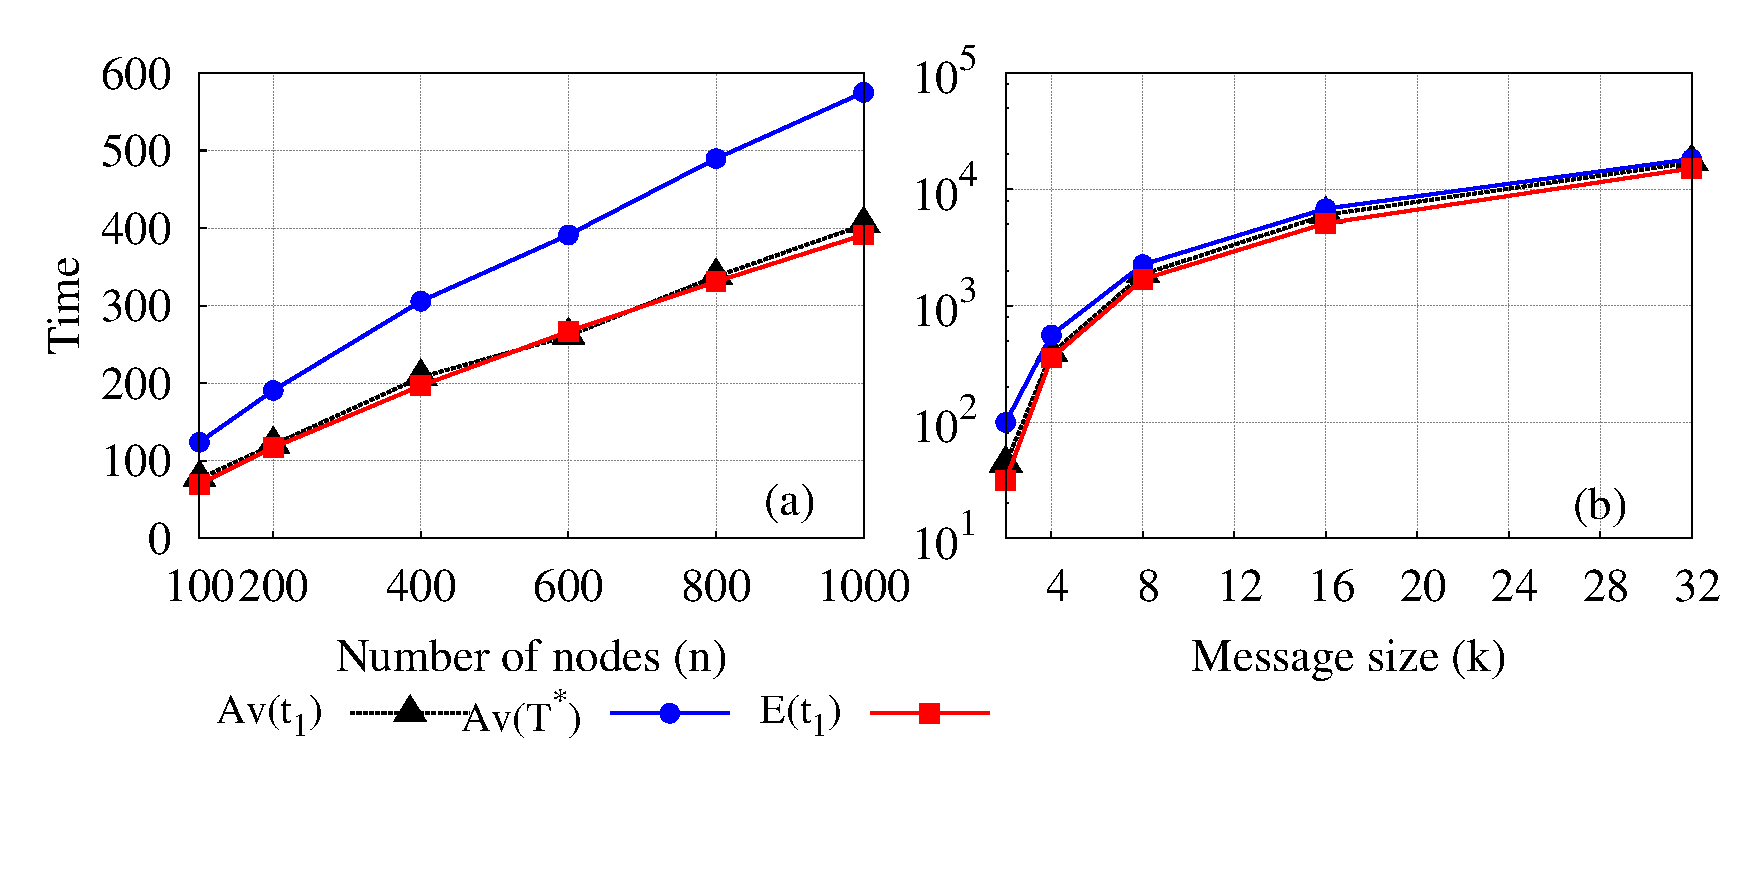
\includegraphics[scale=0.4]{./texfiles/Chapter_3/epl/figs1/plot_var_n_k_complete.eps}
 
 %\vspace{-5mm}
 \caption{$Av(T^*)$ and $Av(t_1)$ versus (a) the number of nodes with message size $k=4$ and (b) $k$ for fixed $d=1000$.
  For both the plots $\hat E(t_1) = C \ast d^{\frac{k-1}{k}}$ where $C = (k!)^{\frac{1}{k}}\Gamma\left(1+\frac{1}{k}\right)$ (refer to theorem \ref{theorem-1}).}
 \label{segSizeVsDelay_nrTrans_varyN_Mall_push_pull}
 %\vspace{-.3cm}
 \end{figure}
% The
% remaining growth is very fast - actually of logarithmic order since several
% new senders in every time step get produced. \vspace{-2mm}

%{\bf E-R Random graphs} - 


\noindent{\em E-R random graph}: We further look into {\bf Erdos-Renyi random graphs}~\cite{erdos1959random} and observe that for sufficiently 
dense graphs (i.e., having high edge probability) the analysis on the complete graph case holds.  
In this regard we first plot $Av(T^{\ast})$ (obtained through simulations) and $\hat{E}(T^{\ast})$ ($n^{\frac{k-1}{k}}$ scaled by a constant, $n$ is the number of nodes) for 
different values of $k$ (message size) (refer to figure \ref{fig_diff_g_n_p}(a)). 
Clearly the theoretical estimate closely follows the simulated result. {As we increase the value of edge probabilities($p$) (i.e., make the network more dense)
 the closer it gets to the theoretical estimate.}
We further plot $Av(T^{\ast})$ (scaled by $\hat{E}(t_{1})$) for varying $p$ in figure \ref{fig_diff_g_n_p}(b). 
The value gets close to 2 with edge probability 1 but remains close to 2 even for lower values of $p$. 
All the results are averaged over $1000$ simulations.



\begin{figure}[htpb]
%\vspace{-.4cm}
\centering
  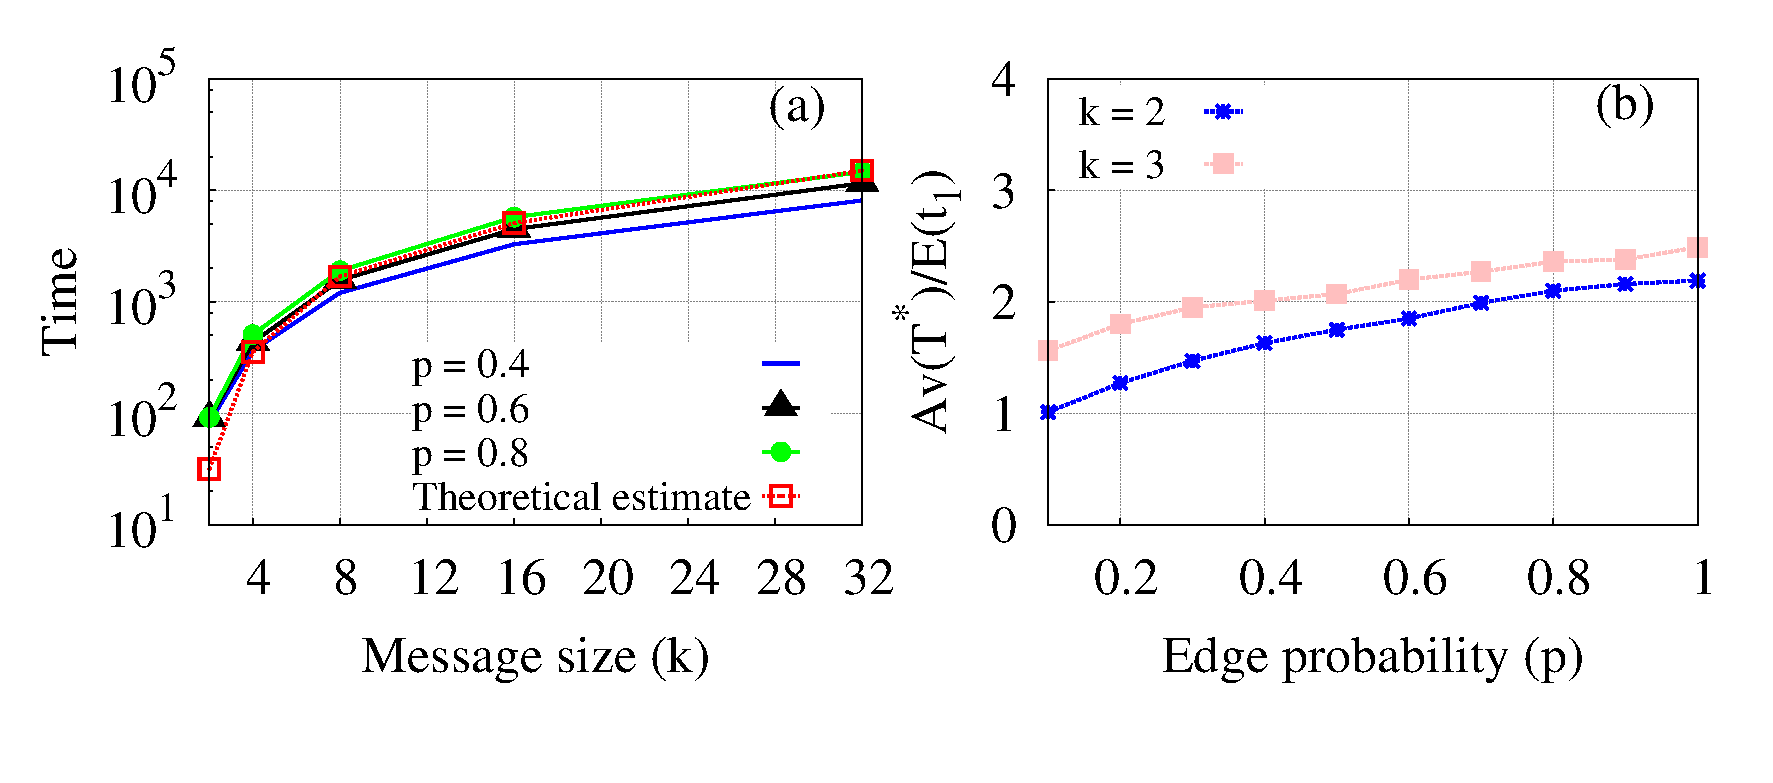
\includegraphics[scale=0.4]{./texfiles/Chapter_3/epl/figs1/ER_graph_result.eps}
  
  %\vspace{-3mm}
  \caption{\label{fig_diff_g_n_p}(a) $Av(T^{\ast})$ and $\hat E(T^{\ast})$ (suitably scaled) for different values of $k$ 
  (b)$Av(T^{\ast})$ versus edge probability in Erdos-Renyi random graph for $k=2$ and $k=3$. In both cases $Av(T^{\ast})$ is normalized by $\hat{E}(t_{1})$ which is $\sqrt{n}$ and $n^{\frac{2}{3}}$ for $k=2$ and $k=3$ respectively.
  \vspace{5mm}}
  %\vspace{-.5cm}
 \end{figure}

%  \begin{figure}[htpb]
%  \centering
%   \includegraphics[scale=0.28]{figs1/tree_ratio.eps}
%   \caption{\label{tree_ratio} ratio of $s_t$ and $s_{t-1}$ throughout the 
% whole duration of the diffusion process for a 5-regular tree }
%  \end{figure} 

\medskip
